\documentclass[thesis.tex]{subfiles}

\title{Estimating duration in the presence of misclassification}
\author{Joshua Blake}
\date{\today}

\begin{document}

\ifSubfilesClassLoaded{
  \setcounter{chapter}{1}
}

\chapter{SARS-CoV-2: biology and data} \label{biology-data}

SARS-CoV-2 is closely related to previous coronaviruses that have caused outbreaks in humans, SARS-CoV and MERS-CoV.
Coronaviruses are RNA (Ribonucleic acid) viruses.
RNA viruses use RNA, rather than DNA, as their genetic material.
RNA viruses, which include influenza, mutate rapidly and are the most likely class of viruses to cause pandemics~\autocite{woolhouseRNA}.

The initial and most sensitive diagnostic test for SARS-CoV-2 uses RT-PCR, which I explain in \cref{biology-data:sec:PCR}.
SARS-CoV-2 causes the disease COVID-19; I discuss the \emph{natural history} of the disease, the course it takes from beginning to end~\autocite[193]{portaEpiDictionary}, in \cref{biology-data:sec:natural-history}.

I then move on to discussing the two studies I use in this thesis.
These are ATACCC (\cref{biology-data:sec:ataccc}) and the CIS (\cref{intro:sec:cis}), both briefly discussed in \cref{E-intro}.
Unlike many studies of SARS-CoV-2, these studies are not focused on specific groups such as healthcare workers or hospital patients.
Therefore, the results from these studies are more generalizable to the entire UK population.

\section{PCR testing} \label{biology-data:sec:PCR}

PCR (Polymerase Chain Reaction) is a procedure that produces millions to billions of copies of a specific segment of DNA (Deoxyribonucleic acid) from a single copy~\autocite{smithPCR,garibyanPCR}.
This is known as \emph{amplifying} the DNA.
PCR has many uses within the biological sciences; Mark R.\ Hughes, deputy director of the Human Genome Project, has claimed it is the most important scientific technology of the last hundred years~\autocite{powledgePCR}.
It is central to the work in this thesis because it can detect the presence of SARS-CoV-2 in a sample taken from a human, most commonly a nose and/or throat swab.

\subsection{Reverse transcription}

SARS-CoV-2 is an RNA virus, but PCR amplifies DNA.
Therefore, before using PCR process to detect SARS-CoV-2, the RNA must be converted to DNA.
This process is known as \emph{reverse transcription}.
In reverse transcription, a naturally occurring enzyme known as reverse transcriptase generates cDNA (complementary DNA) from the RNA in the sample~\autocite{valasekPower}.
Any sequence of cDNA has a one-to-one correspondence with a sequence of RNA.
The cDNA can then be used in the standard PCR process.

\subsection{The PCR process} \label{biology-data:sec:PCR-process}

\todo[inline]{Consider finding or making a figure to explain PCR testing.}

The PCR process requires four substances at its start: template DNA, nucleotides, primers, and DNA polymerase~\autocite{garibyanPCR}.
The \emph{template DNA}, in this context, is the sample which is being tested~\autocite{caseTemplate}.
\emph{Nucleotides} or \emph{bases} are the building blocks of DNA.
There are four nucleotides in DNA (A, C, G, T) each of which forms a pair, known as a \emph{base pair}, with its \emph{complementary} nucleotide (A with T, and G with C)~\autocite{batesBase}.
The choice of \emph{primers} specifies the exact DNA to amplify; they are the complementary DNA sequence to the start and end of the DNA sequence to be amplified~\autocite{garibyanPCR}.
DNA \emph{polymerase} is an enzyme required to link individual nucleotides together~\autocite{garibyanPCR}.

The process is a series of cycles, each cycle containing three steps~\autocite{powledgePCR,garibyanPCR}.
The first step, \emph{denaturation}, heats the DNA causing its two strands to separate.
The second step, \emph{annealing}, lowers the temperature, causing the primers to bind to the DNA.
The final step, \emph{extension}, raises the temperature, causing the DNA polymerase to replicate the DNA sequence between the primers. 
In the course of such a cycle, the amount of DNA doubles.
Therefore, the number of DNA copies increases geometrically with the number of cycles completed.

\emph{Quantitative real-time (RT-)PCR} gives a measurement of the amount of the target DNA sequence present in the original sample~\autocite{yangPCRdiagnostics}.
After each PCR cycle, the amount of target DNA is measured and compared to a pre-derived standard.
Once the measurement exceeds the standard, the target DNA is declared detected. 
The number of cycles required to reach detection is known as the \emph{cycle threshold} (Ct) value.
Originally, measurement occurred only after the completion of all cycles, hence the name real-time.
Quantitative real-time PCR has other practical advantages (\eg speed); see \textcite{yangPCRdiagnostics,valasekPower} for more details.
All RT-PCR tests I consider in this thesis are quantitative real-time RT-PCR tests and produce Ct values.

% The Ct value decreases as the amount of DNA present in the original sample increases~\autocite{hanRTPCR}.
If there is more RNA present, reverse transcription creates proportionally more DNA.
More initial DNA means fewer cycles until detection; that is, the Ct value is lower~\autocite{hanRTPCR}.
The number of DNA copies doubles each cycle, therefore the log Ct value decreases linearly with the quantity of RNA or DNA in the original sample (see \cref{biology-data:fig:ct-calibration}).
A \emph{standard curve} translates the Ct value to viral load for a given test.
A standard curve is produced by measuring the Ct value using reference samples with known viral load, and, as seen in \cref{biology-data:fig:ct-calibration}, they vary between studies.
\begin{figure}
    \centering
    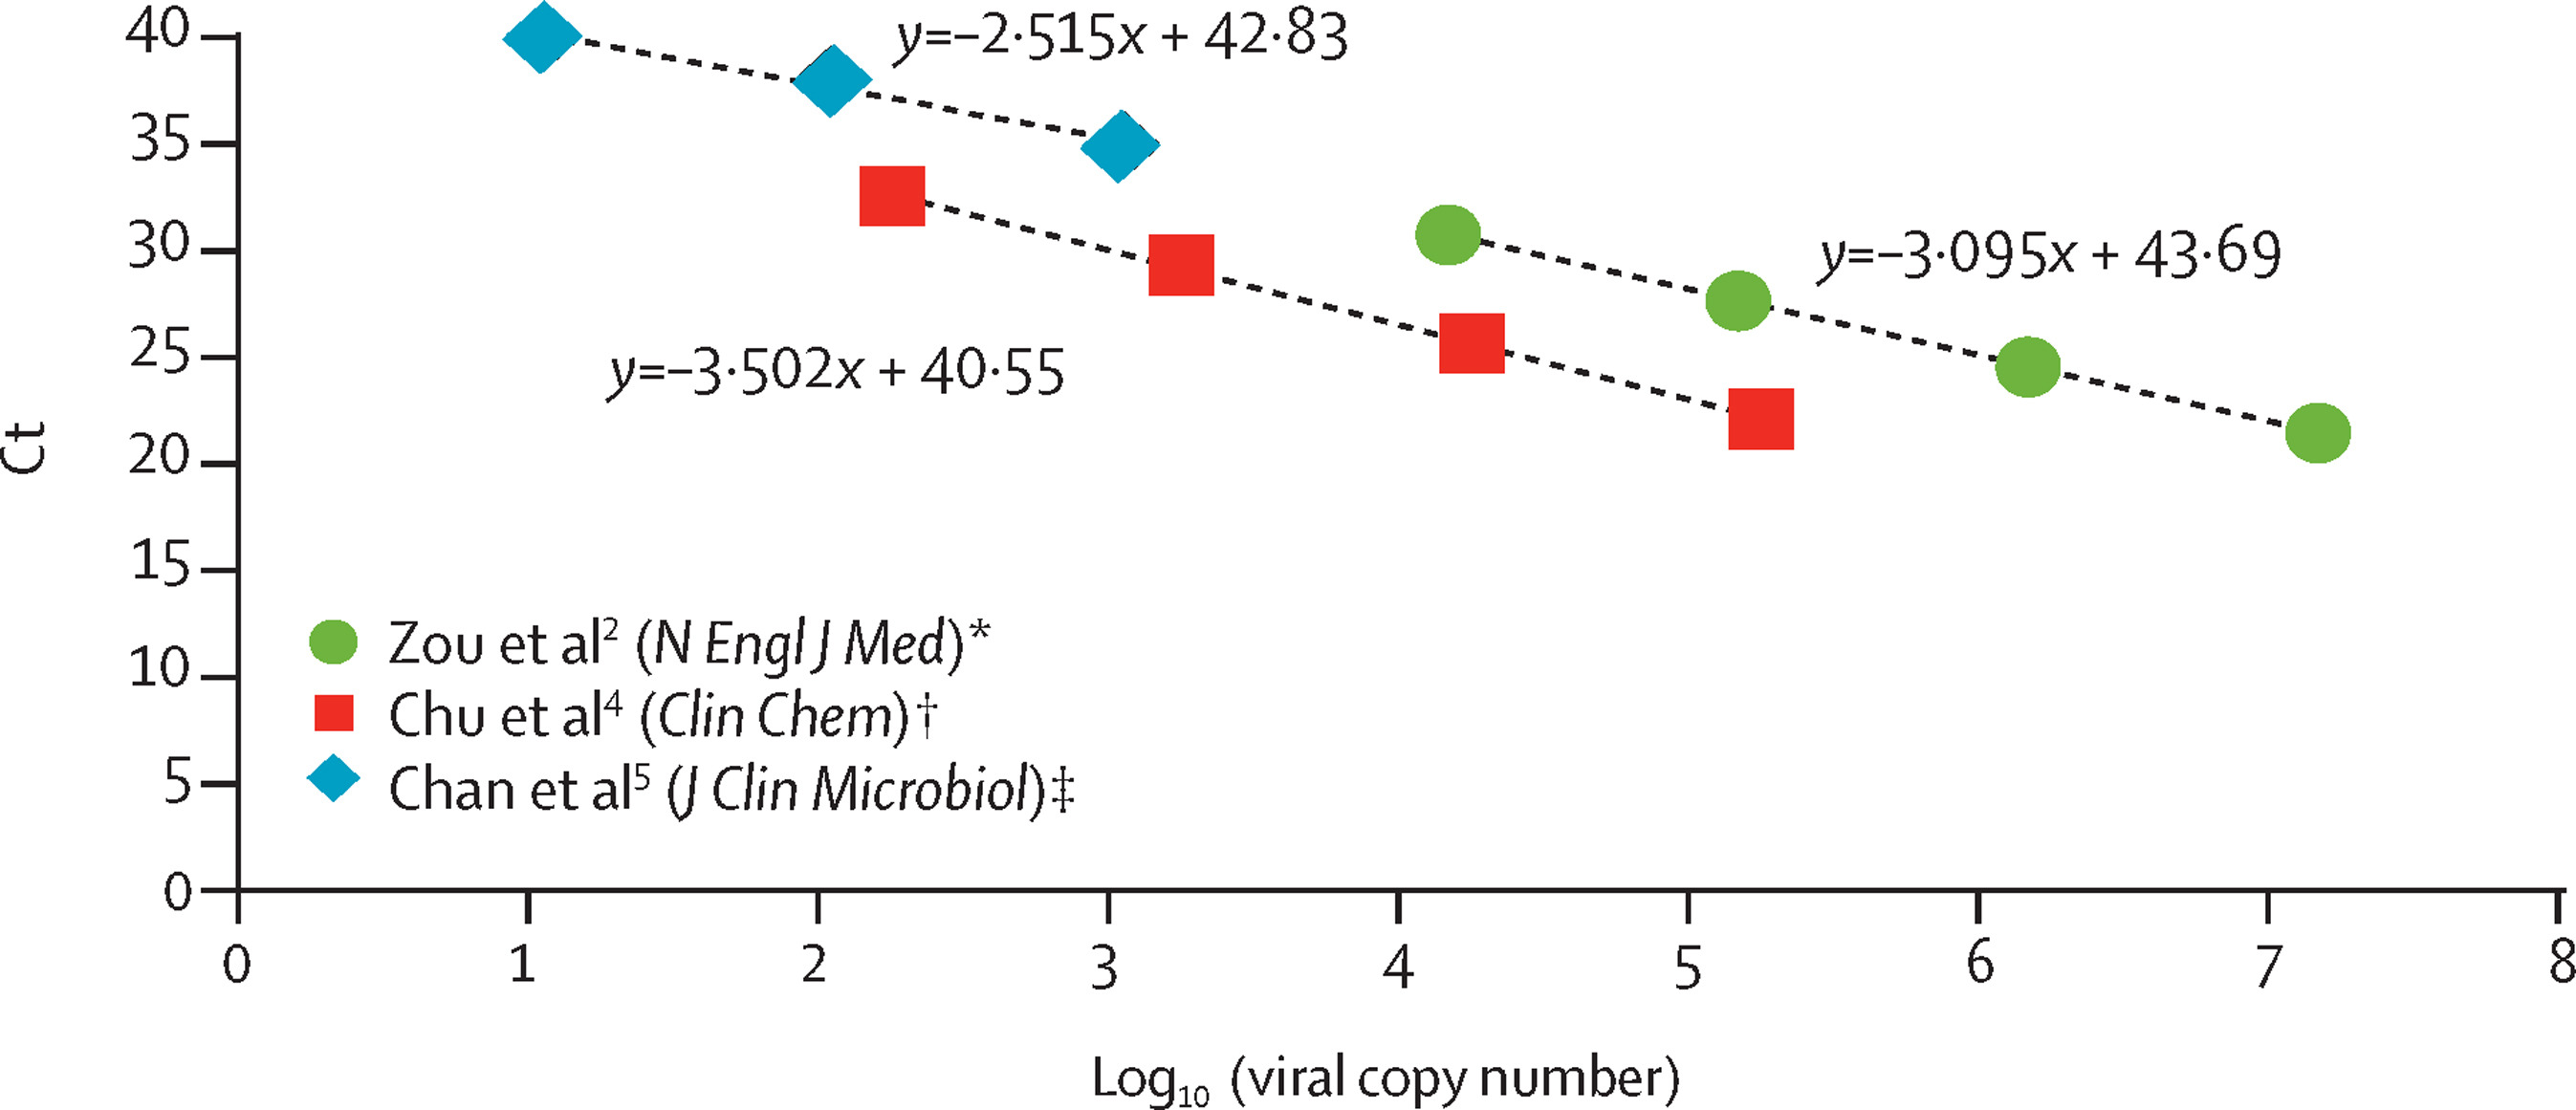
\includegraphics[width=\textwidth]{biology-data/ct-calibration}
    \caption[Example standard Ct curves]{%
        Example standard curves, which relate the logarithm of the viral copy number (the number of copies of the target DNA or RNA in the sample) to the measured Ct value.
        Reproduced from \textcite{hanRTPCR} with permission.
    }
    \label{biology-data:fig:ct-calibration}
\end{figure}

\subsection{Detectable individuals} \label{biology-data:sec:detectable}

An important concept throughout this thesis will be that of \emph{detectable} individuals.
An individual is defined as detectable between the time they would first test positive on a perfect RT-PCR test (if tested) and the time they would stop doing so.
It is not possible to conclusively determine whether an individual is detectable because perfect RT-PCR tests do not exist (see \cref{biology-data:sec:PCR}).
However, viewing the number of RNA genome copies in an individual as a latent process this can then be defined as the time when the number of RNA genome copies is above the limit of detection of the RT-PCR test (defined in \cref{biology-data:sec:measurement-error}).
% While this definition is not perfectly precise, it is clear enough for the purposes it used in this thesis.


\subsection{Measurement error} \label{biology-data:sec:measurement-error}

Like any diagnostic test, PCR tests are not perfect.
The quantitative result (the Ct value) is noisy, and the qualitative result (positive or negative) can be wrong.
Errors arise from a variety of sources, including the sampling/swabbing process and batch effects in the RT-PCR process~\autocite{hanRTPCR}.

The \emph{analytical sensitivity} of the test is the minimum number of copies of the target RNA material in the sample that the test can detect, typically expressed as the \emph{limit of detection}~\autocite{bustinMIQE}.
The limit of detection is the lowest concentration of the target RNA material that can be reliably detected using the procedure; below this level there is a substantial (generally, >5\%) chance that errors in the process cause the amplification procedure to fail~\autocite{forootanLOD}.
This is different to the \emph{clinical sensitivity} of the test, the ability of the test to detect a detectable individual.
Clinical sensitivity is affected by a large variety of preanalytical factors, \eg sample collection (\ie the swabbing process) and sample transportation~\autocite{lippiPotential}.
Clinical sensitivity is of primary interest in this thesis.
I will quantify it as the \emph{test sensitivity} (strictly the clinical test sensitivity), the probability of a positive test result for a detectable individual.
A negative result for a detectable individual is a \emph{false negative}.

The \emph{analytical specificity} of the test is the ability of the test to distinguish between the intended target rather than other, non-specific RNA (or DNA) sequences present in the sample~\autocite{bustinMIQE}.
As with sensitivity, this is different to the \emph{clinical specificity} of the test, the ability of the test to distinguish between detectable and undetectable individuals.
A positive result for an undetectable individual is a \emph{false positive}.

False positives are very rare for SARS-CoV-2 RT-PCR tests.
In summer 2020, the CIS performed 208,730 PCR tests and found only 159 positives~\autocite[section 5]{cisMethodsONS}.
If these were all false positives, then the test specificity would be 99.9\%.
In reality, it is almost certain that some of these are true positives, and hence this is a lower-bound on the true test specificity.

RT-PCR enables the detection of SARS-CoV-2 viral RNA in a sample.
However, this does not necessarily mean that the virus is viable (\ie able to reproduce, a necessary condition for transmission to occur)~\autocite{puhachSARSCoV2}.
Determining viability requires more sophisticated tests, although high viral loads (low Ct values) are positively correlated with viability.
The gold standard procedure for assessing viability is attempting to grow and recover viral material from a sample, a process known as \emph{cell culturing}~\autocite{singanayagamDuration,puhachSARSCoV2,hakkiOnset}.
Further details on cell culturing are beyond the scope of this thesis.

\section{Natural history of the disease} \label{biology-data:sec:natural-history}

\begin{figure}
  \makebox[\textwidth][c]{
  \begin{tikzpicture}[
      node distance = 4cm,
      on grid,
      auto,
      ->,>=stealth',
      every state/.style={draw,rectangle,align=center},
      ]

      \node[state] (pre) {RT-PCR negative \\ Not infectious};
      \node[state, right of=pre] (pos) {RT-PCR positive \\ Not infectious};
      \node[state, right of=pos] (infectious) {RT-PCR positive \\ Infectious};
      \node[state, right of=infectious] (not-infectious) {RT-PCR positive \\ Not infectious};
      \node[state, right of=not-infectious] (neg) {RT-PCR negative \\ Not infectious};

      \node[draw=none, below=2cm of pre] (infected) {} ;
      \node[draw=none, below=2cm of neg] (recovered) {} ;

      \node[above=2cm of pre] (titleA) {(A)};
      \node[below=1cm of infected] (titleB) {(B)};

      % \draw (0,-2) -- node {Infected} (pre);
      % \draw (not-infectious) -- (0,-2);

      \path (infected) edge node {Infected} (pre)
          (pre) edge (pos)
            (pos) edge (infectious)
            (infectious) edge (not-infectious)
            (not-infectious) edge (neg)
            (neg) edge (recovered);
    
    % Detectable
    \node[below = 1cm of infectious] (detect-label) {Detectable};
    \node[draw, thick, inner sep=0.3cm, fit=(pos) (infectious) (not-infectious) (detect-label), fill=red!10,opacity=0.3] (detect-box) {};
  \end{tikzpicture}
  }
  \centering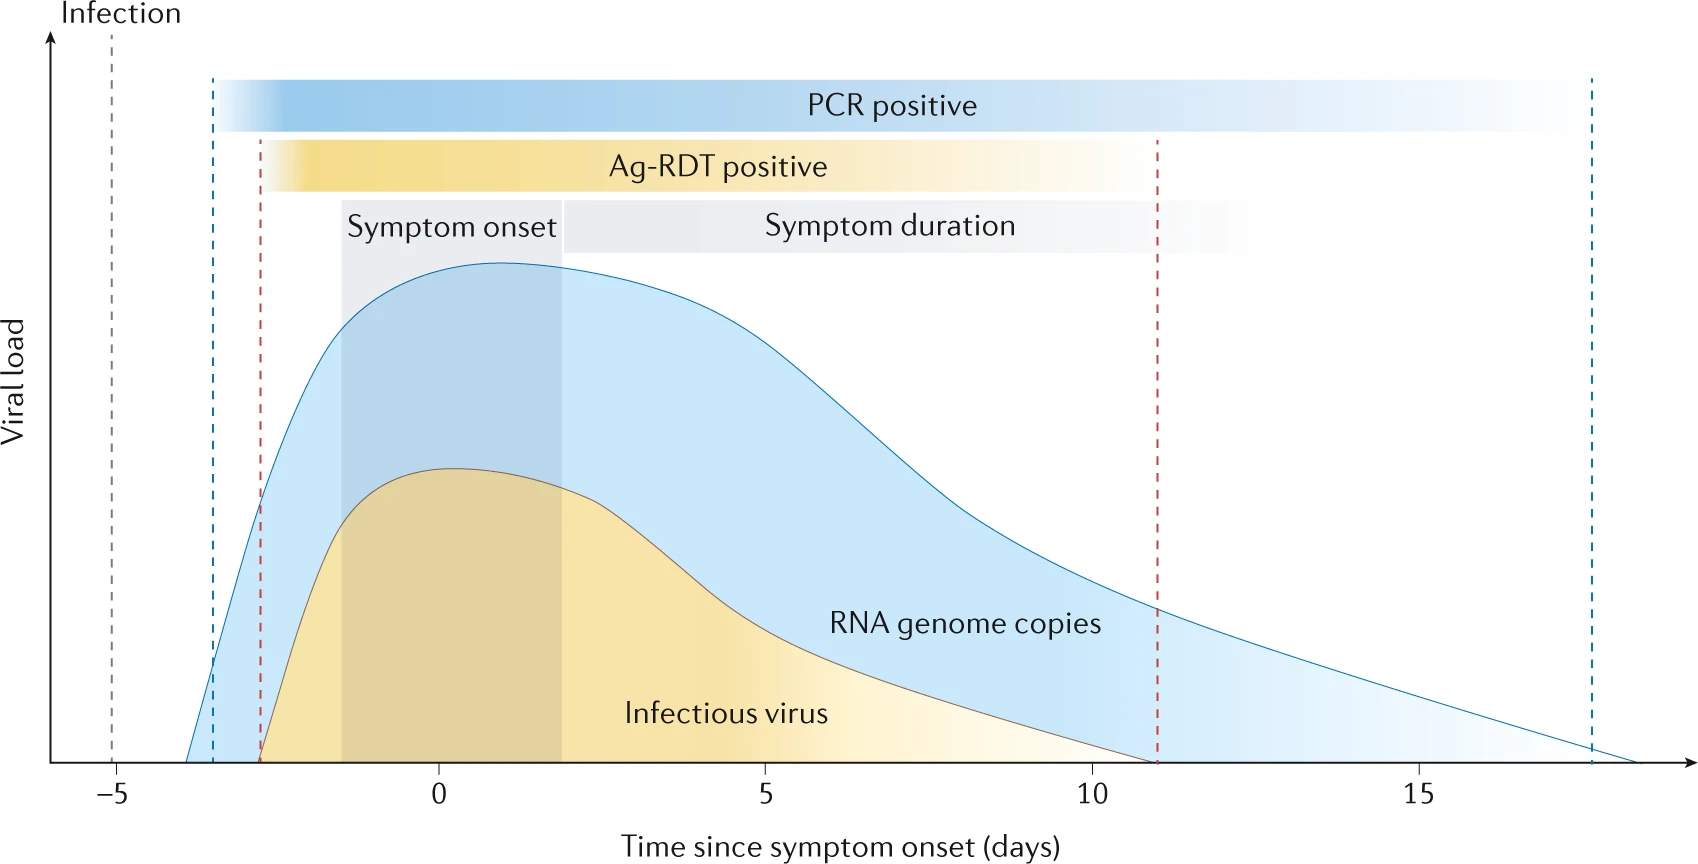
\includegraphics[width=\textwidth]{biology-data/natural-history}
  \caption[Natural history of SARS-CoV-2.]{%
    Natural history of SARS-CoV-2.
    (A) A simplified state-based representation of the natural history.
    Shading represents states where the individual is detectable by an RT-PCR test.
    (B) A fuller representation of the natural history, including the latent processes of the quantity of RNA genome copied and infectious virus within and individual (reproduced from \textcite{puhachSARSCoV2} with permission).
    Ag-RDT (antigen rapid diagnostic test) tests are lateral flow tests, which detect infectious virus rather than RNA, and are not used in this thesis.
  }
  \label{biology-data:fig:natural-history}
\end{figure}

An individual infected with SARS-CoV-2 goes through several disease stages, depicted in \cref{biology-data:fig:natural-history}~\autocite{puhachSARSCoV2}.
First, the individual is exposed to the virus and becomes infected.
At this initial stage they are not infectious (cannot spread the disease to others), do not have symptoms, and will not test positive on an RT-PCR test.
After a few days, they will start testing positive on an RT-PCR test; this is normally prior to being infectious or having symptoms.
Next, the individual becomes infectious; normally, this occurs prior to symptom onset for those who experience symptoms.
Recovery from symptoms occurs after a few days, around the time the individual is no longer infectious.
Finally, the individual will test negative on an RT-PCR test.

The time for each of these stages depends on various features of host and virus characteristics and has a large amount of variation.
In this thesis, I focus on pre-Alpha variants of SARS-CoV-2 in unvaccinated individuals.
The time from infection to infectiousness is known as the \emph{latent period}.
The length of the latent period is hard to estimate because we rarely observe either the time of infection or the start of infectiousness.
Estimates of its length are based on careful contact tracing, where transmission times are thought to be known with a reasonable degree of certainty.
These estimates vary but suggest a mean length of 3--4 days for pre-Alpha variants~\autocite[and references therein]{zhaoEstimating}.
The time from infection to experiencing symptoms is known as the \emph{incubation period}; it is undefined for asymptomatic individuals.
As the symptom onset time (when symptoms start) is often known, this is easier to estimate than the latent period.
However, the unknown infection time still poses challenges, again requiring contact tracing data.
Therefore, estimates are sensitive to the choice of data and statistical model.
Its mean length is around 6 days~\autocite{wuIncubation,quesadaIncubation,aleneSerial}.

A host's \emph{viral load}, the quantity of viral particles in a host, is the underlying biological process driving the different periods and characteristics of an infection~\autocite{puhachSARSCoV2}.
Any host's viral load is determined by the interaction of many biological processes, most prominently the virus's replication increasing the viral load and the host's immune response reducing the viral load~\autocite{keVivo}.
Viral replication requires the virus to infect a host cell and then use the host cell's machinery to produce more virus; as more host cells are infected this process slows because there are fewer remaining potential host cells, known as \emph{target cells}, to infect.
Host cells which can potentially be infected are known as \emph{target cells}.
The rate at which host cells are infected slows over time because there are fewer remaining target cells to infect.
The host's immune system can slow this process by various mechanisms; the most relevant for SARS-CoV-2 is by making some target cells less susceptible to infection.
A host's immune response is triggered by the viral load and becomes stronger as the viral load increases.
A high viral load is associated with being more infectious, more likely to test positive on an RT-PCR test, and the start of symptoms~\autocite{puhachSARSCoV2,keVivo}.


% Possible summaries
% \begin{enumerate}
%   \item \url{https://www.nature.com/articles/s41579-022-00822-w/figures/2}
%   \item \url{https://www.nature.com/articles/s41576-021-00360-w/figures/1}
%   \item \url{https://academic.oup.com/view-large/figure/305617142/ciaa1442_fig2.jpg}
% \end{enumerate}


% \section{Studies used ie this thesis} \label{biology-data:sec:studies}

% In this section, I expand on the major two studies I use in this thesis (ATACCC and CIS).
% Unlike many studies of SARS-CoV-2, these studies are not focused on specific groups such as healthcare workers or hospital patients.
% Therefore, the results from these studies are more generalisable to the entire UK population.


\section{Assessment of Transmission and Contagiousness of COVID-19 in Contacts} \label{biology-data:sec:ataccc}

The ATACCC study was a longitudinal study of contacts reported to the NHS Test and Trace contact tracing service~\autocite{hakkiOnset}.
Contacts were invited to participate if they were 5 years or older and  could be reached within 5 days of the index case's symptom onset date.
ATACCC enrolled a total of 738 contacts across two waves.
The first wave enrolled 393 contacts between 13th Sep 2020 and 31st Mar 2021, when pre-Alpha and Alpha variants were circulating.
The second wave enrolled 345 contacts between 24th May 2021 and 228th Oct 2021, when the Delta variant was circulating.
Contacts were swabbed daily for up to 20 days, with a variety of tests performed on the swabs; relevant for this thesis is the RT-PCR test for SARS-CoV-2.
For all positive test results, the viral load was measured using the Ct value and then converted to a viral load using a standard curve (see \cref{biology-data:sec:PCR-process}).
Other data such as demography and symptoms were also collected, although I do not use this information.
For further details see \textcite{singanayagamDuration,hakkiOnset}.

Of the 738 contacts enrolled, 172 (23\%) had at least one positive test
\Textcite{hakkiOnset} analysed the 57 contacts who tested positive for SARS-CoV-2 and had the growth phase in their viral load measured.
They excluded the remaining 115 contacts with at least one positive RT-PCR test, ATACCC did not capture the phase of the infection with increasing viral load.
This exclusion was to ensure viral load trajectories are identifiable.
I will revisit and extend this analysis in \cref{E-ATACCC}.

\section{Coronavirus (COVID-19) Infection Survey} \label{intro:sec:cis}

The CIS~\autocite{CIS} was set up in April 2020 to provide gold-standard measurements of the prevalence of SARS-CoV-2 in the community.
It was a longitudinal study with a representative sample of private households, \ie excluding settings such as care homes and student halls.
The dataset is globally unique in providing a representative, longitudinal, and large-scale study across the pandemic.
Initially, it was limited to England, but expanded to cover the whole of the UK in September 2020.
Enrolment was continuous until 31st Jan 2022, with data collected until 13th Mar 2023~\autocite{weiRisk}. 

The CIS had a household-based design, meaning that households were invited to participate in the study.
From households that participated, all individuals aged 2 and over were invited to participate.
Once invited, an enrolment swab would be taken at the first visit followed by 4 further weekly visits (giving a total of 5 swabs on days 0, 7, 14, 21, 28 relative to enrolment) after which visits were monthly.
As well as a swab to test for SARS-CoV-2, participants were asked to complete a questionnaire, and some participants were asked to provide blood samples.
In reality, visits were often not on this precise schedule, and occasionally missed.
A full description of the study can be found in the study protocol~\autocite{cisProtocol}.

Up until July 2020, households were selected from those that had previously participated in an ONS survey~\autocite{CIStechData}.
Around 50\% of households agreed to participate, with around 90\% of eligible individuals (96,113 in total) in these households contributing multiple swabs to the survey.
After July 2020, addresses were also randomly sampled from a database of all UK addresses held by the ONS.
The response rate was lower, with only 12\% of households agreeing to participate, from which 86\% of eligible individuals (383,732 in total) contributed multiple swabs to the survey.

These rates of response raise the possibility of non-response bias.
In particular, some demographic groups, such as young adults and individuals of non-White ethnicity, were underrepresented among those who responded~\autocite{pouwelsCommunity}.

In this thesis, I focus on the period from Mon 31st Aug 2020 until Sun 24th Jan 2021 (see \cref{E-intro:sec:aims}).
During the start of this period, the recruitment rate of CIS was expanded (see \cref{biology-data:fig:CIS-recruitment}(A)).
Following this, the recruitment then decreases and stabilises, as does the rate of swabs taken (see \cref{biology-data:fig:CIS-recruitment}(B)).
The recruitment pattern was chosen to hit targets regarding the fortnightly number of swabs.
Because testing becomes less frequent after the first 4 weeks, some continuous recruitment is needed to maintain the number of swabs, as well as to replace participants who drop out.

\begin{figure}
  \centering 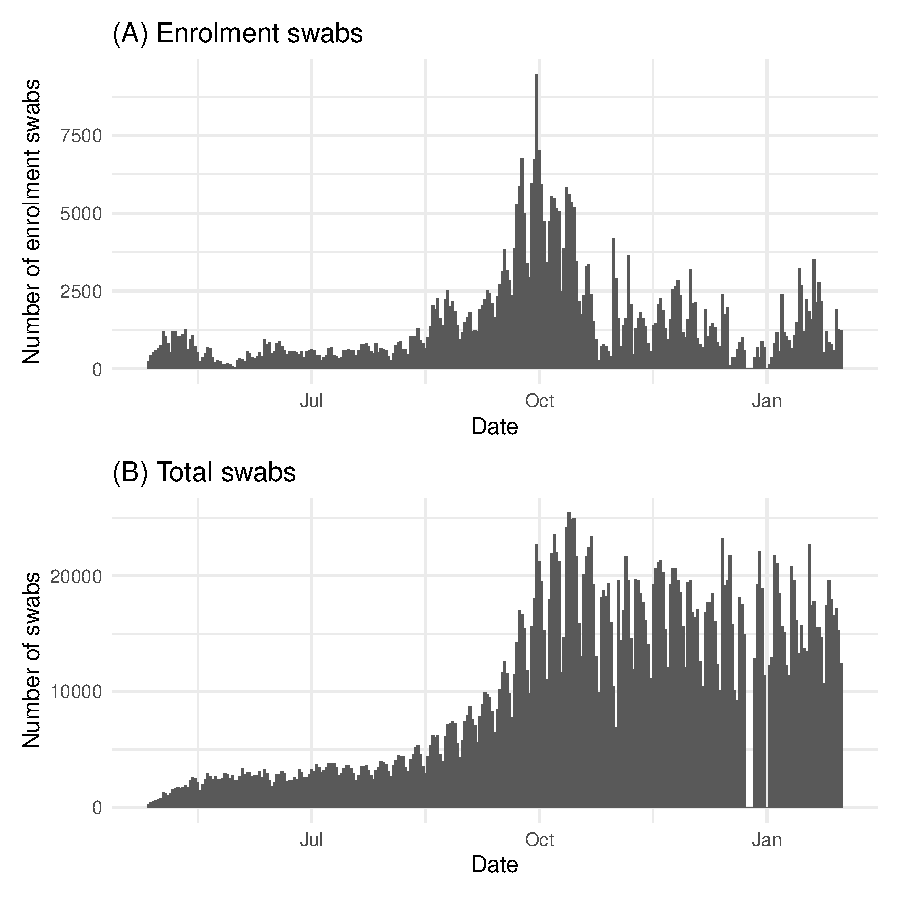
\includegraphics{biology-data/CIS-recruitment}
  \caption[CIS swab numbers]{%
    Number of swabs taken by the CIS in the period considered in this thesis (Sep 2020 until Jan 2021).
    (A) Only enrolment (\ie first) swabs for each individual.
    (B) Total swabs.
    Note the differing y-axis scales.
    Data from \textcite{CIStechData}.
  }
  \label{biology-data:fig:CIS-recruitment}
\end{figure}
% \begin{figure}
%   \centering 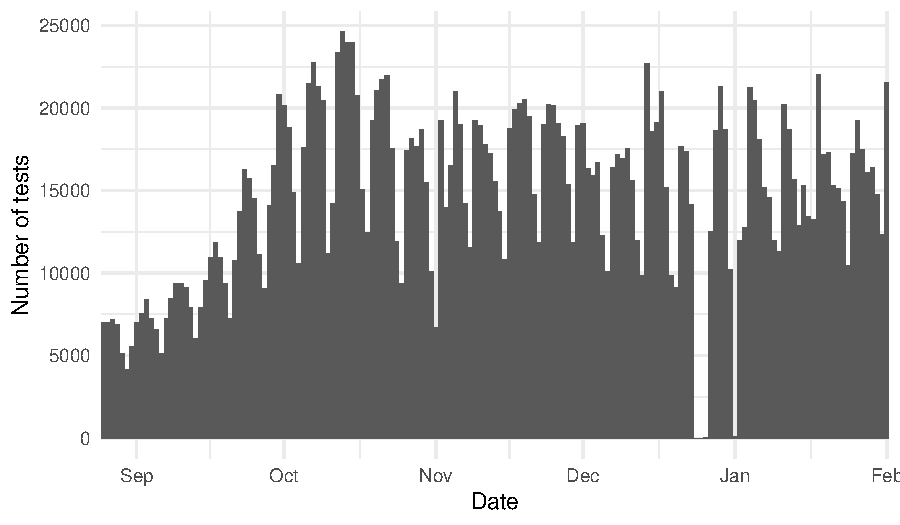
\includegraphics[width=\textwidth]{biology-data/CIS-num-tests}
%   \caption[Number of CIS tests]{%
%     Daily number of CIS tests conducted in the period considered in this thesis (Sep 2020 until Jan 2021).
%   }
%   \label{biology-data:fig:CIS-num-tests}
%   \todo[inline]{Cut this repetition of number of tests? Maybe highlight period of interest in previous plot}
% \end{figure}


The main result reported by the study was what they defined as the \emph{positivity rate}, the proportion of people in a given (sub)population that (if they were tested using RT-PCR) would test positive for SARS-CoV-2 at a defined point in time~\autocite{cisMethodsONS}.
A notable feature of this definition is that it explicitly does not correct for false positive or negative results.
However, for many purposes, including this thesis, the difference between the positivity rate and prevalence is negligible.

Generally, the point in time of interest is a specific day, although it has also been applied to a week~\autocite{cisMethodsONS,pouwelsMRPvaccination,pouwelsCommunity}.
Larger time periods (\ie weeks instead of days) allow more granular estimates in other dimensions, most commonly geography.

\subsection{Strata} \label{biology-data:sec:cis-strata}

In estimating positivity, I will divide the population into strata based on age group, sex, ethnicity, and geographic area.
I will report results aggregated to geographic regions and age groups, as done previously.
For the purposes of both fitting and reporting results, test results are aggregated into daily counts for each stratum.

The age groups used have varied slightly for different CIS analyses~\autocite[e.g.][]{pouwelsMRPvaccination,pouwelsCommunity,cisMethodsONS,houseInferring,walkerTracking}.
I will use the age groups: 0--10 (pre-school and primary school), 11--15 (compulsory secondary school), 16--24 (adolescents and young adults who may remain in formal education), 25--49 (younger working age adults), 50--69 (older working age adults), and 70+ (elderly).

I use two levels of ethnic grouping.
Broad groupings (White and non-White), because the White population makes up a large majority of the UK.
I also use more granular ethnicities (Asian, Black, Mixed, White, and Other).

The geographic areas I will adopt are the nine standard regions of England (International Territorial Level 1, previously Nomenclature of Territorial Units for Statistics 1); these are: North East, North West, Yorkshire and the Humber (commonly abbreviated to Yorkshire), East Midlands, West Midlands, East, London, South East, and South West~\autocite{onsRegions}.
These are the geographic areas used throughout the major CIS analyses in England, although sometimes more granular areas were defined~\autocite[e.g.][]{pouwelsMRPvaccination,pouwelsCommunity,cisMethodsONS,houseInferring,walkerTracking}.

\subsection{Adjustment for non-response and data sparsity} \label{biology-data:sec:MRP}

If the CIS was truly a random sample, an unbiased estimator of the positivity rate would be the proportion of positive tests in the sample; I refer to this estimator as the unadjusted positivity rate.
However, in practice, two issues arise with this.
First, the non-response bias discussed previously.
Second, the number of positives on any day is low, especially among any specific subpopulation (\eg age group or region).
Statistical methods are used to correct for these issues.

The preferred statistical method for estimating the positivity rate is MRP (multi-level regression and poststratification)~\autocite{cisMethodsONS,pouwelsCommunity}.
MRP is a statistical methodology developed to correct political opinion polling suffering from response bias~\autocite{gelmanMRT,gelmanPoststratication,parkMRP}.
MRP is a two-step process.
In this context, the first step, multilevel regression, consists of using a Bayesian multilevel logistic regression model to predict RT-PCR test results in the sample based on demographic covariates.
To address the low number of positives, MRP uses a hierarchical Bayesian model to borrow information across time and other covariates.
The second step, poststratification, uses the posterior distribution of the parameters predict the population prevalence in each stratum.
These are combined by taking a weighted average across the strata, where a stratum's weight is equal to its (known) population size.
The poststratification step corrects for non-response bias.

I modified the regression component of a pre-existing version of a MRP model for CIS~\autocite{pouwelsMRPvaccination}, as recommended by that model's author for the specific context of this thesis~\citePersonalComms{Koen Pouwels}.
As in prior work~\autocite{pouwelsMRPvaccination}, I used INLA for inference, implemented in R-INLA (see \cref{E-transmission:sec:INLA}).
For a day $t$, age group $a$, ethnicity $e$, and sex $s$ the regression model is:
\begin{align}
    \logit(p_{taes}) &= \beta + \beta_s + \beta_{w(e)} + u_a + v_e + w_t + l_{a,t} \\
    y_{taes} &\dist \BB(n_{taes}, p_{taes}, \rho).
\end{align}
The terms are as follows.
\todo[inline]{Check I've written the priors correctly}
\begin{itemize}
    \item $n_{taes}$ and $y_{taes}$ are the number of individuals tested and the number of positive test results on day $t$ in individuals of age group $a$, ethnicity $e$, and sex $s$. I use a beta-binomial distribution, as discussed in \cref{biology-data:sec:clustering}.
    \item $\beta$ is a global intercept term with the vague prior $\beta \dist \N(0, 1/0.001^2)$.
    \item $\beta_s$ is a fixed effect for sex, with $\beta_s = 0$ for males and estimated for females. The prior for $\beta_s$ is vague, $\beta_s \dist \N(0, 1/0.001^2)$.
    \item $\beta_{w(e)}$ is a fixed effect for White or non-White ethnicity. $\beta_{w(e)} = 0$ if $e$ corresponds to White ethnicity and $\beta_{w(e)} = \beta_{n}$ otherwise (\ie non-White ethnic groups).
      The prior for $\beta_n$ is vague, $\beta_n \dist \N(0, 1/0.001^2)$.
      % $\beta_n$ and $\beta_f$ have the default INLA prior for fixed effects\todo{check what this is}.
    \item $u_a$ and $v_e$ are independent normal random effects for age and ethnic group respectively. Their standard deviation has a penalized complexity prior~\autocite{simpsonPenalising} with a 10\% probability of being greater than 1.
    \item $w_t$ is a second-order random walk, that is $w_t = 2w_{t-1} - w_{t-2} + \epsilon_t$ where $\epsilon_t \dist \N(0, \sigma_w^2)$.
      $\sigma_w$ has a vague prior, $1/\sigma_w \dist \GamDist(1, 5 \times 10^{-5})$.
    \item $l_{a,t}$ is an age-group specific second-order random walk.
      That is $l_{a,t} = 2l_{a,t-1} - l_{a,t-2} + \epsilon_{a,t}$ where $\epsilon_{a,t} \dist \N(0, \sigma_l^2)$.
      $\sigma_l$ has a vague prior, $1/\sigma_l \dist \GamDist(1, 5 \times 10^{-5})$.
\end{itemize}
For parameters given vague priors, the large amount of data means that the prior has little influence on the posterior distribution.
The second-order random walk priors favours linear growth in $\logit(p_{taes})$ over time.
For the small values of $p_{taes}$ likely to be encountered, this approximates exponential growth.

I fitted the model separately and independently for each region, implicitly adding all interactions between region and the other variables.
This step assumes that the estimates for each region can be considered independent, which is reasonable because the regions are large with many tests conducted within each.

The final step is poststratifying the incidence proportion to the CIS target population and subpopulations of interest.
To start, I draw a sample of 500 prevalence time series in each stratum from the approximate posterior distribution (using the procedure described in \cref{transmission:sec:INLA:posterior}).
For each posterior draw and day, the incidence proportion in the (sub)population is the weighted average of the incidence proportion in each stratum, where the weights are the number of individuals in that stratum.
The population numbers for each stratum are provided by the Office for National Statistics.

\subsection{Clustering} \label{biology-data:sec:clustering}

The household-based design of the CIS means that the data is clustered.
In particular, individuals in the same household are likely to transmit to each other and hence have correlated test results.
Other behavioural or genetic factors could also contribute to individuals in the same household being more similar than randomly selected individuals in the population.
The positivity analyses use a beta-binomial likelihood (defined in \cref{E-distributions}) to account for this.

The beta-binomial distribution is overdispersed relative to the binomial distribution.
Overdispersion allows for household clustering and other overdispersion in the data, which is common in epidemiological data~\autocite{griffithsBBD}.
The parameterization of the beta-binomial that I use (detailed in \cref{E-distributions}) has an overdispersion parameter $\rho$, regarded as a nuisance parameter in this context.
$\rho=0$ means the beta-binomial coincides with the binomial distribution.
As $\rho \to \infty$, the distribution tends towards the uniform distribution on $[0, 1]$~\autocite{hughesUsing}.

\subsection{Positivity results} \label{biology-data:sec:positivity-results}

\Cref{biology-data:fig:CIS-positivity} shows estimates from this model compared to the unadjusted positivity rate.
Both show similar trends.
The MRP estimate most often increases the estimated positivity rate, compared to uncorrected positivity rate, because the underrepresented demographic groups tended to have higher positivity rates.

\begin{figure}
  \centering 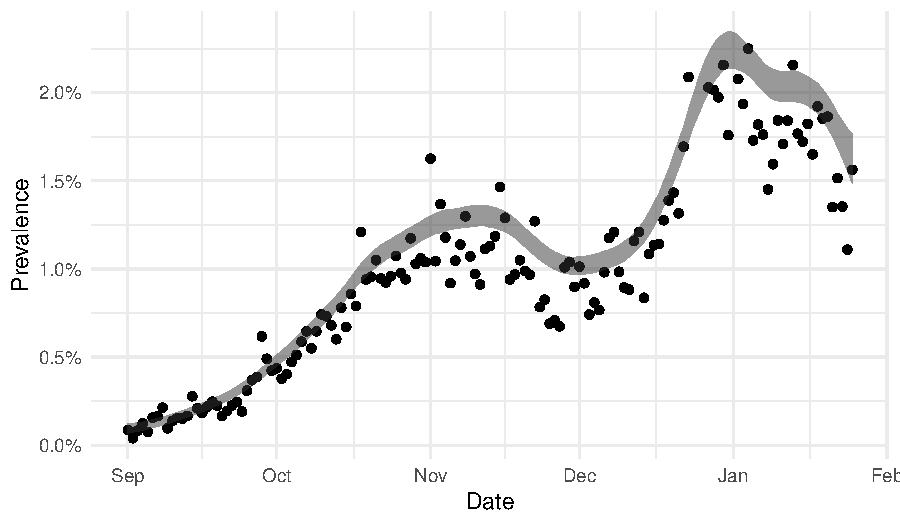
\includegraphics[width=\textwidth]{biology-data/CIS-positivity}
  \caption[CIS positivity]{%
    CIS positivity rate in the period considered in this thesis (Sep 2020 until Jan 2021).
    Dots show the unadjusted positivity rate (days with fewer than 100 tests are excluded for readability).
    Ribbon shows modelled 95\% CrI for the positivity, corrected for non-response bias and smoothed over time (using the methodology described in \cref{E-backcalc:sec:methods}).
  }
  \label{biology-data:fig:CIS-positivity}
\end{figure}


\subsection{Episodes} \label{biology-data:sec:cis-episodes}

Positive test results need to be grouped into \emph{infection episodes}.
An infection episode is a series of positive tests that originate from a single transmission event.
I use a heuristic-based algorithm developed throughout the pandemic and published within \textcite{weiRisk}; see that publication for full justification of the criteria.

The algorithm determines whether a new positive test, at time $t$, is part of the previous infection episode in the same individual.
If the individual has no previous positive tests, the new positive test is always the start of a new infection episode.
Otherwise, denote the first positive test associated with that previous infection episode as $t_p$, and the number of negative tests immediately prior to the test at $t$ as $n$.
The test at $t$, in the pre-Omicron era (prior to December 2021), is defined as the start of a new infection episode if any of the following apply.
\begin{enumerate}
  \item $n \geq 1$ and $t - t_p > 120$.
  \item $n \geq 2$ and $t - t_p > 90$.
  \item $n \geq 3$ and $t - t_p > 60$.
  \item $n \geq 4$.
  \item A complex heuristic based on the likely variant of the positive tests (see \textcite{weiRisk} for details). This heuristic rarely applied in the pre-Omicron era~\citePersonalComms{Sarah Walker}.
\end{enumerate}

A negative between two positive tests, when those positives are part of the same infection episode, is known as an \emph{intermittent negative}.
Intermittent negatives are the clearest example of a false negative.
I will generally consider that intermittent negatives are uninformative on the duration of detectability, and hence exclude them from several analyses.

A sample of 500 randomly selected infection episodes (selected from the episodes used in the analyses in this thesis) have their test results shown in \cref{biology-data:fig:episodes}.
The number of tests within an episode, their length, and other characteristics vary greatly.
\begin{figure}
  \thisfloatpagestyle{empty}
  \vspace{-5cm}
  \makebox[\textwidth][c]{
\includegraphics[height=.7\paperheight]{biology-data/STATS13734/data_viz}}
  \caption[CIS infection episodes]{%
    500 randomly selected infection episodes.
    Shown are the negative tests before and after the outermost positive tests associated with the episode.
    Red dots are negative tests, green dots are positive tests, and blue dots are void tests (where the result could not be determined; excluded from other analyses).
  }
\end{figure}

The crucial features of an infection episode are the start and end times of the infection.
Ignoring misclassified test results, latent start time of infection episode $j$, $B_j$, can be bounded as between the day after the last negative test, $l_j^{(b)}$, and the day of the first positive test, $r_j^{(b)}$.
Similarly, the latent end time of infection episode $i$, $E_j$, can be bounded as between the day of the last positive test, $l_j^{(e)}$, and the day before the following negative test, $r_j^{(e)}$.

\subsection{Computational limitations and privacy protection} \label{biology-data:sec:SRS}

For privacy reasons, the CIS data is stored in the ONS's SRS (Secure Research Service)~\autocite{onsSRS}.
The SRS is a Trusted Research Environment (TRE) that allows researchers to access sensitive data in a secure environment.
The SRS gives accredited researchers working on projects in the public interest access to granular data which cannot be legally shared publicly.

Statistical disclosure controls must be applied to any data or results to be extracted from the SRS.
Statistical disclosure control ensures that no individual can be identified from the data.
This means that data must be aggregated to counts of at least 5, and no individual-level data included.

Analyses requiring more fine-grained stratification (such as that in \cref{biology-data:sec:MRP}) or linking data from the same individual over time (such as that in \cref{E-perf-test,E-imperf-test}) must be performed within the SRS.
Therefore, computationally efficient approaches must be taken to this work.
The SRS contains limited computational power.
It has\todo{insert SRS computational power}.
However, these are shared computational resources and due consideration must be given to other users.
Processes which run for multiple days are liable to be cancelled.

This computational limitation will feature in several places in this thesis.

\section{Conclusion}

In this chapter, I have introduced RT-PCR testing, the natural history of SARS-CoV-2, and the two studies used in this thesis.
The next chapter will introduce the data generating processes behind infection, prevalence, and our observations of these processes.
Then, I will apply these concepts to the two studies.


\ifSubfilesClassLoaded{
  \listoftodos
}{}

\end{document}